\documentclass{article}

\usepackage{tikz}
\usetikzlibrary{positioning}


\begin{document}
% STYLES
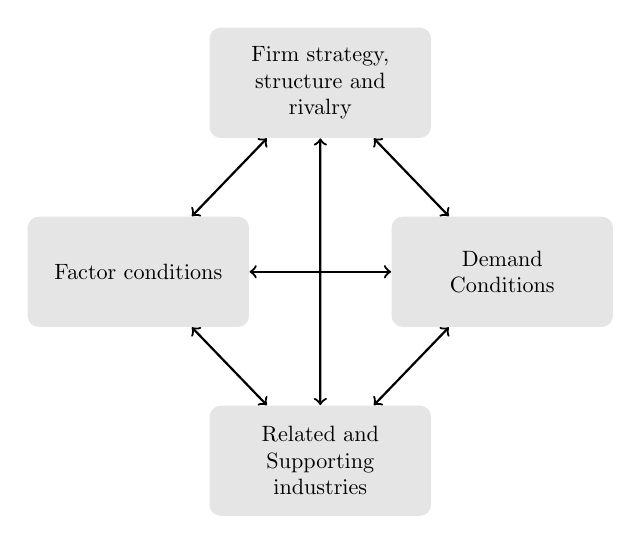
\begin{tikzpicture}[scale=0.8,transform shape]
% STYLES
\tikzset{%
    force/.style={%
        rectangle,rounded corners, minimum width=100pt,
        align=center,node distance=3cm,fill=black!10,inner sep=5pt,
        text width=3cm,minimum height=1.75cm,>=stealth,text badly centered
    }
}
% Draw forces
\node (rivalry) {};% was missing!!
\node [force, above of=rivalry] (top) {Firm strategy, structure and rivalry};
\node [force, left=1cm of rivalry] (left) {Factor conditions};
\node [force, right=1cm of rivalry] (right) {Demand Conditions};
\node [force, below of=rivalry] (bottom) {Related and Supporting industries};
% Draw the links between forces
\path[<->,thick]
    (left) edge (right)
    (left) edge (top)
    (left) edge (bottom)
    (top) edge (right)
    (bottom) edge (right);
\path[<->,thick] (bottom) edge (top);
\end{tikzpicture}


\end{document}